\documentclass[12pt,a4paper]{article}

%% ─── Packages ────────────────────────────────────────────────────────────────
\usepackage[top=1in,bottom=1in,left=1.1in,right=1.1in]{geometry}
\usepackage{amsmath,amssymb}
\usepackage[hidelinks]{hyperref}
\usepackage{enumitem}
\usepackage{xcolor}
\usepackage{float}
\usepackage{tikz}
\usetikzlibrary{arrows.meta,positioning,shapes.geometric,calc}
\usepackage{setspace}
\usepackage{parskip}
\usepackage{titlesec}
\usepackage{microtype}
\usepackage{graphicx}
\usepackage{booktabs}
\usepackage{array}
\usepackage{fancyhdr}

%% ─── Spacing ─────────────────────────────────────────────────────────────────
\onehalfspacing
\setlength{\parindent}{0pt}
\setlength{\parskip}{0.65em}

%% ─── Colours ─────────────────────────────────────────────────────────────────
\definecolor{mainblue}{RGB}{25,95,175}
\definecolor{lightblue}{RGB}{218,232,252}
\definecolor{darkgray}{RGB}{60,60,60}
\definecolor{arrowgray}{RGB}{110,110,110}
\definecolor{nodered}{RGB}{190,50,30}
\definecolor{nodegreen}{RGB}{30,140,80}
\definecolor{lightyellow}{RGB}{255,250,220}
\definecolor{lightgreen}{RGB}{220,248,230}

%% ─── Section headings ────────────────────────────────────────────────────────
\titleformat{\section}
  {\large\bfseries\color{mainblue}}
  {\thesection.}{0.55em}{}
  [\vspace{0.1em}{\color{mainblue!50}\rule{\linewidth}{0.6pt}}]

\titleformat{\subsection}
  {\normalsize\bfseries\color{darkgray}}
  {\thesubsection}{0.6em}{}

\titlespacing*{\section}{0pt}{1.6em}{0.6em}
\titlespacing*{\subsection}{0pt}{1em}{0.3em}

%% ─── Header / footer ─────────────────────────────────────────────────────────
\pagestyle{fancy}
\fancyhf{}
\renewcommand{\headrulewidth}{0.3pt}
\fancyhead[L]{\small\color{darkgray} Knowledge-Graph-Driven Multilingual Educational Platform}
\fancyhead[R]{\small\color{darkgray} BTP Report · IIIT Hyderabad}
\fancyfoot[C]{\thepage}


%% ═══════════════════════════════════════════════════════════════════════════
\begin{document}
\thispagestyle{empty}

%% ─── Title Page ─────────────────────────────────────────────────────────────
\begin{center}
\vspace*{1.2cm}
{\large\bfseries International Institute of Information Technology, Hyderabad}\\[1.4cm]

{\color{mainblue}\rule{\linewidth}{1.8pt}}\\[0.8cm]

{\LARGE\bfseries A Knowledge-Graph-Driven\\[0.45cm]
Multilingual Educational Platform\\[0.45cm]
for Indian School Curricula}\\[0.8cm]

{\color{mainblue}\rule{\linewidth}{1.8pt}}\\[2.2cm]

{\large B.Tech Project (BTP)}\\[0.35cm]
{\large Academic Year 2025--2026}\\[2.6cm]

\renewcommand{\arraystretch}{1.9}
\begin{tabular}{c@{\qquad\qquad\quad}c}
  \textbf{\large Saksham Chitkara} & \textbf{\large Swam Singla} \\
  {\normalsize Roll No.\ 2023101021} & {\normalsize Roll No.\ 2023101134}
\end{tabular}

\vspace{1.2cm}
{\normalsize Advisor: \textbf{Prof.\ Vasudeva Varma}}\\[0.3cm]
{\normalsize IIIT Hyderabad}

\vfill
{\large May 2026}
\end{center}

\newpage
\thispagestyle{plain}

%% ─── Abstract ────────────────────────────────────────────────────────────────
\begin{abstract}
\noindent
India has over 250 million school students, the vast majority of whom learn in regional
languages rather than English.
Yet high-quality, curriculum-aligned educational content in Indic languages is almost
entirely absent from digital platforms.
This project builds a multilingual educational platform for school Mathematics and Science,
covering Grades~6 through~12 across NCERT, ICSE, and several state boards.

The project evolved through two major phases.
The first phase extracted sections directly from official textbook PDFs,
generated explanations using a locally hosted language model,
and translated them into Hindi, Telugu, and Odia through a neural translation pipeline.
This produced working results but revealed a deep structural flaw: organising content
by textbook chapter rather than by concept led to inconsistency, redundant generation,
broken translation of mathematical notation, and no meaningful navigation between related ideas.

The second phase rebuilt the system from the ground up around a \emph{knowledge graph}:
a directed network of canonical concepts linked by prerequisite relationships.
Every concept is defined and generated exactly once.
Content is grounded in the original textbooks through Retrieval-Augmented Generation (RAG),
and produced directly in all four languages using Sarvam~AI models,
eliminating the translation step entirely.
The result is a web platform where any concept in the curriculum (from Whole Numbers in
Grade~6 to Differential Equations in Grade~12) is one click away from everything the
student needs to know before it and everything it enables next.
\end{abstract}

\tableofcontents
\newpage

%% ═══════════════════════════════════════════════════════════════════════════
\section{Introduction}

India runs one of the largest school education systems in the world,
with hundreds of millions of students across thousands of schools.
Yet the digital resources available to those students are almost entirely in English,
and high-quality regional language content for school Mathematics and Science is largely absent.

The existing digital landscape for school education presents a consistent set of limitations:

\begin{itemize}[leftmargin=2em, itemsep=0.3em]
  \item Most free content available online is in English. Regional language material,
    where it exists, is typically a translation of English source text rather than content
    written natively for the regional language learner.
  \item Official digital platforms that put textbooks online retain the same linear,
    chapter-based organisation as the printed book. There is no concept navigation,
    no links between related topics across chapters, and no way for a student to identify
    which foundational idea they are missing.
  \item Paid platforms are typically designed for competitive examination preparation.
    They are expensive, examination-focused rather than concept-focused,
    and regional language support beyond Hindi is limited.
  \item Free international platforms offer better concept structure and prerequisite maps,
    but are built around foreign curricula and are not well aligned with Indian boards.
\end{itemize}

The gap this project fills is specific: a free, multi-board educational platform covering
Mathematics and Science for Grades~6 through~12, structured around the actual relationships
between concepts, with content that a student can read in their own language and that
genuinely builds from what they already know toward what they are trying to learn.

This report describes the complete development of that platform: the first version,
what went wrong with it, the redesign it led to, and the system that resulted.

%% ═══════════════════════════════════════════════════════════════════════════
\section{Phase~1: The Chapter-Based Pipeline}

\subsection{Overview}

The first version of the system was designed around the most natural available structure:
the textbook itself.
NCERT books are organised into chapters, chapters into numbered sections,
and sections into content.
The pipeline followed this structure exactly: extract each section from the PDF,
generate an explanation, translate it into regional languages, and serve it.

This produced a working product reasonably quickly,
but the two central choices, chapter as the unit of organisation
    and translation as the path to regional language content, both turned out to be wrong.
The problems they caused were not bugs to be fixed; they were consequences of the design.

\subsection{Extracting Structure from Textbook PDFs}

PDF files store drawing instructions rather than semantic structure, so headings must be
inferred from visual cues such as font size and weight.
The extractor identified the dominant body-text font for each document and treated text
in a substantially different font as a candidate heading, assembling each chapter's
section hierarchy without hardcoding rules for individual textbooks.
This hierarchy became the skeleton the rest of the pipeline operated on.

\subsection{Generating Explanations with a Language Model}


The model used throughout was Meta's LLaMA~3.1~8B Instruct. Before generating a full explanation for a section,
the model first scored the section's importance on a scale of one to five.
This score determined the depth of content generated:
introductory sections received brief summaries while core concepts
received comprehensive explanations with multiple worked examples.
The actual textbook text for the section was provided to the model as context,
keeping the generated content grounded in the curriculum.

The tone and depth were calibrated to grade level.
For Grades~6 to~8, the prompt requested friendly, accessible language with everyday
analogies and encouragement.
For Grades~9 and~10, it requested a balance of accessibility and mathematical precision.
For Grades~11 and~12, it requested rigorous treatment appropriate for students
preparing for national-level university entrance examinations.

Each page followed a consistent structure: an introduction, a main explanation with
worked examples and formatted mathematical expressions, a section on common mistakes,
and a summary.
All mathematical notation was written in standard \LaTeX{} format so it could be rendered
as properly typeset symbols in the browser.

\subsection{Translating into Regional Languages}

Generated English content was then translated into Hindi, Telugu, and Odia.
Three translation model families were implemented, compared, and made available
for selection.

\medskip
\noindent\textbf{IndicTrans2 (AI4Bharat)} supports all 22 scheduled Indian languages
and is fast to generate, but produced lower output quality overall.

\medskip
\noindent\textbf{Sarvam Translate (Sarvam AI)} is built on the Gemma~3 architecture.
It was slower but produced noticeably better results, with more natural phrasing
and better handling of educational terminology across all three languages.
Sarvam was selected as the primary model for the pipeline.

\medskip
\noindent\textbf{TranslateGemma (Google)} was similarly fast to generate
but produced weaker quality output compared to Sarvam.

\medskip
The most technically challenging aspect of the translation pipeline was preserving
mathematical notation.
If a sentence containing a \LaTeX{} formula is sent to a neural translation model,
the model treats the markup as text and typically corrupts, partially translates,
or removes it.
The solution was to split each sentence at formula boundaries before translation:
text segments were sent to the model, and \LaTeX{} expressions were passed through
untouched on a separate path.
After translation, the segments were reassembled.
This preserved mathematical content correctly in the large majority of cases.

Generated and translated content was stored in a cloud-hosted database.
The web application served this content at addresses structured as
Grade $\rightarrow$ Subject $\rightarrow$ Chapter $\rightarrow$ Section.

\subsection{Problems Identified}

After running the full pipeline and examining the output systematically,
three fundamental problems became clear.

\medskip
\noindent\textbf{Mathematical notation was corrupted in translation.}
Neural translation models treat \LaTeX{} markup as text.
A sentence with a formula, sent to a translation model
would often have the formula altered, partially translated, or dropped entirely.
The segment-split workaround (passing formulas through untouched on a separate path)
helped but could not handle all cases, particularly formulas embedded mid-sentence
without clear boundaries.
Students receiving translated content with broken mathematical expressions
were worse off than having no translation at all.

\medskip
\noindent\textbf{Translation terminology was inconsistent within the same subject.}
Each translation run made independent decisions about technical vocabulary.
The Hindi term for ``coefficient,'' ``derivative,'' or ``equilibrium'' might differ
between one section and the next, because the model had no memory across runs.
For subjects where consistent use of terminology is essential to building understanding,
this produced a confusing and unreliable experience across pages.

\medskip
\noindent\textbf{There was no navigation between related concepts.}
A student reading about polynomial equations had no link to algebraic expressions
or factorisation, even though both are directly relevant.
The only navigation was back to the chapter list.
The structure was the same flat, linear arrangement as the printed textbook,
with no improvement in discoverability or context.

\medskip
All three problems pointed to the same underlying causes:
the chapter was the wrong unit of organisation,
and translation was the wrong path to regional language content.

%% ═══════════════════════════════════════════════════════════════════════════
\section{The Core Insight}

The Phase~1 problems share two roots.
The first is structural: the textbook chapter is a publishing artefact,
not a principled representation of knowledge.
It groups material for print convenience, not because the grouped ideas form a coherent unit.
The second is methodological: generating content in English and then translating it
cannot produce high-quality regional language educational material.
Translation is always a lossy second step, and for such content with complex
notation and domain-specific terminology, the losses compound.

The fix to the first problem is to make the \emph{concept} the fundamental unit.
``Quadratic Equations'' is not a section in a Grade~9 textbook.
It is a concept in mathematics, with prerequisites that precede any textbook
that introduces it, and consequences that appear in textbooks years later.
When a concept is the unit, it is defined once and generated once.
Every page knows what the student already understands (its prerequisites)
and can build on that explicitly.
Navigation follows naturally: every concept links to what it depends on
and what it enables.

The fix to the second problem is to eliminate translation entirely.
Instead of generating in English and converting, the system generates content
directly in each target language from the same source material.
A model generating in Hindi applies a consistent internal vocabulary for every
mathematical and scientific term across every concept page it produces.
There is no conversion step in which notation can be corrupted or terminology can drift.
The content is native to its language from the moment it is created.

These two changes, concept as unit and native generation as method, are the foundation of Phase~2.

%% ═══════════════════════════════════════════════════════════════════════════
\section{Phase~2: The Knowledge Graph}

\subsection{Gathering Topics Across Boards}

The first task in Phase~2 was assembling a complete, multi-board topic inventory
for each grade and subject.
NCERT headings from Phase~1 provided the ground-truth baseline,
but topics exclusive to ICSE, Karnataka, Maharashtra, or Andhra Pradesh/Telangana
state boards needed to be identified and included so students from any board
would find their curriculum represented.

The same LLaMA~3.1~8B model handled this stage.
Its breadth of world knowledge made it well suited for curriculum analysis tasks.

The model processed NCERT headings alongside ICSE syllabi and state board course descriptions.
It identified topics common across all boards and topics unique to specific boards.
It also resolved naming inconsistencies: the same concept appearing under different names
in different boards was identified and merged under a single canonical name.
Fuzzy string matching caught near-matches automatically,
and the model resolved ambiguous cases.

This produced a comprehensive raw topic inventory for each grade and subject:
a complete picture of what students across all major Indian boards are expected to learn.

\subsection{Constructing Canonical Concepts}

Raw topic lists from textbooks contain topics at inconsistent levels of granularity.
A chapter heading might cover a broad area; a sub-section heading might name a
narrow technique within it.
Mixing both in the same graph produces nodes at very different scales,
making navigation incoherent.

The goal was to identify canonical concepts at a uniform level of granularity,
similar to the level at which an encyclopedia article would exist.
``Fractions'' is a canonical concept; ``adding fractions with unlike denominators''
is a technique within it.
``Integration'' is a canonical concept; ``integration by substitution'' is an approach
within it, but it also warrants its own concept page because students search for it
and it has its own prerequisites.

The LLM processed raw topic lists and proposed canonical concept names, groupings,
and which of a set of defined mathematical or scientific areas each concept belongs to.
These proposals were carefully reviewed and refined.
The review was a substantial effort, particularly for senior secondary topics where
the right level of abstraction is not always obvious, and the model's suggestions
needed correction in a number of places.

\subsection{Building Prerequisite Edges}

With canonical concepts established, the next step was defining the prerequisite
relationships: for each concept, which other concepts must a student already understand?

The LLM was prompted with a concept and the full candidate concept list,
and asked to identify necessary prerequisites.
These suggestions were reviewed and corrected.
Getting edges right matters.
A missing edge fails to flag a real dependency and leaves a student confused without
knowing why.
A spurious edge implies unnecessary review and disrupts natural learning flow.

The resulting graph is a \emph{directed acyclic graph (DAG)}, a network of directed
arrows representing ``must understand before'' relationships, with no cycles.
A cycle would imply that concept~A requires concept~B which requires concept~A,
a logical impossibility.
The graph was validated computationally using a graph analysis library after every addition.
Any cycle detected indicated an error in the prerequisite assignments, which was
traced and corrected.
Every edge was also verified to point to an existing concept, catching naming errors immediately.

\begin{figure}[H]
\centering
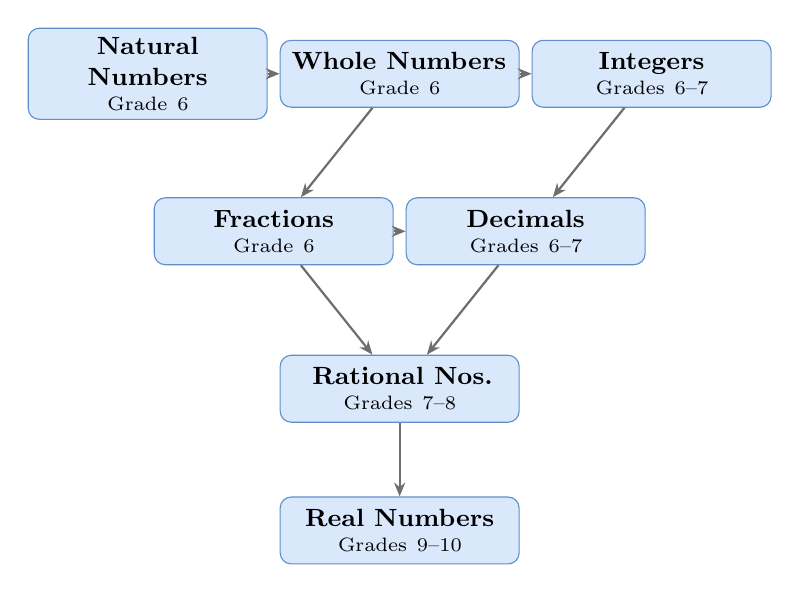
\begin{tikzpicture}[
  cnode/.style = {
    rectangle, draw=mainblue!70, fill=lightblue,
    rounded corners=4pt, text width=2.8cm,
    minimum height=0.85cm, align=center, font=\small\bfseries
  },
  arr/.style = {-{Stealth[length=5pt,width=4pt]}, thick, arrowgray}
]
  \node[cnode] (nat)   at (0,0)      {Natural Numbers\\[-2pt]\scriptsize\normalfont Grade~6};
  \node[cnode] (whole) at (3.2,0)    {Whole Numbers\\[-2pt]\scriptsize\normalfont Grade~6};
  \node[cnode] (int)   at (6.4,0)    {Integers\\[-2pt]\scriptsize\normalfont Grades~6--7};
  \node[cnode] (frac)  at (1.6,-2.0) {Fractions\\[-2pt]\scriptsize\normalfont Grade~6};
  \node[cnode] (dec)   at (4.8,-2.0) {Decimals\\[-2pt]\scriptsize\normalfont Grades~6--7};
  \node[cnode] (rat)   at (3.2,-4.0) {Rational Nos.\\[-2pt]\scriptsize\normalfont Grades~7--8};
  \node[cnode] (real)  at (3.2,-5.8) {Real Numbers\\[-2pt]\scriptsize\normalfont Grades~9--10};

  \draw[arr] (nat)   -- (whole);
  \draw[arr] (whole) -- (int);
  \draw[arr] (whole) -- (frac);
  \draw[arr] (int)   -- (dec);
  \draw[arr] (frac)  -- (dec);
  \draw[arr] (frac)  -- (rat);
  \draw[arr] (dec)   -- (rat);
  \draw[arr] (rat)   -- (real);
\end{tikzpicture}
\caption{A portion of the Number Systems subgraph.
         Each arrow means ``must understand before.''
         Concepts span multiple grade levels and the graph spans from Grade~6 through Grade~12.}
\label{fig:numsubgraph}
\end{figure}

\subsection{Manual Expert Curation}

A substantial part of the graph was built through manual curation rather than automated
generation alone.
Each concept was defined explicitly: its canonical name, the grades it covers,
which area it belongs to, its prerequisites, and a description of what the concept is.
The graph was rebuilt and re-validated computationally with every addition.
Prerequisite relationships can appear obvious but be wrong in subtle ways that would
mislead students; the manual curation pass ensured the graph is educationally sound throughout.

The Mathematics graph spans Grades~6 through~12 across eighteen areas including Number Systems,
Algebra, Geometry, Trigonometry, Calculus, Statistics, and Probability, with cross-area
prerequisite links wherever concepts from different areas genuinely depend on each other.
The Science graph covers Physics, Chemistry, and Biology across the same grade range,
and includes cross-subject edges to the Mathematics graph where scientific topics
directly require mathematical tools.
Together, the two graphs cover the complete school curriculum across all major Indian boards.

%% ═══════════════════════════════════════════════════════════════════════════
\section{Content Generation}

\subsection{Grounding Generation in the Knowledge Graph}

Generating educational content purely from a language model's parametric knowledge
is unreliable for a curriculum-aligned system.
Models produce explanations that sound authoritative but contain subtle errors:
wrong formula applications, imprecise definitions, and reasoning steps
that deviate from the curriculum.
The solution in Phase~2 is to assemble a rich context for every concept
before any content is generated, drawing from three complementary sources.

The first source is the knowledge graph itself.
For every concept and grade, the graph is traversed to extract the canonical names
and descriptions of prerequisite concepts (what the student must already understand),
the concepts this page unlocks (what it enables next),
and related concepts in the same mathematical or scientific area.
This structural context tells the generator exactly what prior knowledge it can build on,
what it does not need to re-explain, and what future material it can naturally foreshadow.

The second source is the original NCERT textbooks.
Textbook content is stored as short passages and matched to each concept
by comparing the concept's name against passage titles and content.
The best-matching passages are included in the generation context,
giving the model access to the actual textbook language rather than relying on
its internal knowledge alone.

The third source is externally fetched reference material for additional factual grounding,
particularly useful for higher-grade concepts where textbook coverage is less complete.
All three sources are assembled into a single structured context before any API call is made,
ensuring that every generated page is grounded simultaneously in the curriculum structure,
the textbook content, and broader subject knowledge.

\subsection{Direct Multilingual Generation via Sarvam~AI}

Phase~1 generated content in English and ran a separate translation pass.
Phase~2 eliminates translation entirely.
For each concept and grade, content is generated in English, Hindi, Telugu, and Odia
as four separate generation calls, all using the same assembled context.
Sarvam~AI models handle the Indic language runs, large language models trained with
a strong emphasis on Indian languages and Indian educational content.

Each generation call receives the full structured context:
the concept's name, area, grade, and description;
the prerequisite concepts with their descriptions so the model knows what the student
already understands and need not be re-explained;
the list of concepts this one unlocks, for natural foreshadowing;
related cross-links drawn from the graph;
the matched textbook passages and reference material;
and a grade-calibrated depth instruction that sets the appropriate level of rigour and detail.
For Indic language runs, the model is instructed to write entirely in the target script,
with mathematical notation in standard \LaTeX{} as the only Latin-character content.

Mathematical notation is embedded directly in the generated content by the model itself,
in all four languages.
Because formulas are produced in the generation step rather than passed through
a translation layer, there is no possibility of corruption.
The same formula appears identically across every language version of a concept page.

Terminology consistency follows automatically from native generation.
A model generating in Hindi applies its internally learned vocabulary for
mathematical and scientific terms uniformly across every concept it produces.
There is no independent translation decision per page and no post-processing
required to standardise terms across the curriculum.

%% ═══════════════════════════════════════════════════════════════════════════
\section{The Web Platform}

The platform consists of a Next.js web application and an Express API server,
with all content stored in a cloud-hosted database.
Concept pages are pre-rendered as static HTML at build time,
so they load immediately on any connection without any server computation at request time.
All four language versions of every page are pre-rendered in the same way.

Navigation follows the structure of the knowledge graph.
Students begin at a subject hub (Mathematics or Science) which displays the areas the subject
is divided into and links to grade-level views.
From a grade view, all concepts taught at that grade are shown grouped by area.
On any concept page, the student sees the concept's area and grade context,
a short description, the list of prerequisites (each linking directly to its own page),
the full generated explanation with properly typeset mathematical notation,
and the list of concepts this one unlocks.
A student can follow prerequisite links backwards to find exactly where a gap in their
understanding lies, or follow successor links forward to see what a mastered concept enables.

Every concept page is available in English, Hindi, Telugu, and Odia.
A language selector switches the explanation to the chosen language.
Mathematical notation is identical across all language versions because it was generated
alongside the language content, not translated separately.

A global search bar finds concepts by name, area, or description across all grades and subjects.
Concepts with no prerequisites at a given grade are highlighted as natural entry points,
guiding students who are beginning a new grade toward where to start.

%% ═══════════════════════════════════════════════════════════════════════════
\section{Discussion}

\subsection{What Phase~1 Taught Us}

The Phase~1 pipeline was built and run in full before being abandoned.
This was not wasted effort.
Running it produced concrete evidence of exactly what failed and why,
which made the design of Phase~2 well-grounded rather than speculative.

The three problems identified in Phase~1 (broken mathematical notation in translation,
terminology inconsistency across sections, and absence of concept navigation)
all traced to two root causes: the chapter was the wrong abstraction,
and translation was the wrong path to regional language content.
Recognising this clearly, rather than patching around it, justified the substantial
effort of rebuilding from scratch.

\subsection{The Knowledge Graph as an Educational Artefact}

The knowledge graphs built in this project are not just data structures for the software system.
They are educational artefacts in their own right.

Building them required thinking carefully about what every topic in the school curriculum
actually depends on and what it enables, questions that textbooks leave implicit
but which have real answers.
Working through every concept across seven grades in two subjects produced a structure
with genuine educational value beyond the software it supports.

The graph also surfaces the cross-subject connections that curricula typically leave implicit:
where science topics depend directly on specific mathematical tools,
those links are made explicit, so students can see both the scientific and mathematical
prerequisites of any concept.

%% ═══════════════════════════════════════════════════════════════════════════
\section{Conclusion}

This project built a multilingual educational platform for Indian school students
that does not exist elsewhere in free form: concept-structured, multi-board,
covering Mathematics and Science for Grades~6 through~12,
with content generated directly in English, Hindi, Telugu, and Odia.

The path involved building a first version, identifying its failures precisely,
understanding those failures as design problems rather than implementation bugs,
and redesigning from scratch around the correct abstraction.
The knowledge graph, the core artifact of Phase~2, is the result of that redesign.

The platform gives a student something no digitised textbook can:
a map of what they are trying to learn.
Every concept they encounter has a page that shows them what they need to know before it
and where it leads afterward.
They can follow that map in any direction, in their own language,
with explanations grounded in the textbooks their curriculum uses.

The result is a tool that treats learning as the interconnected, cumulative, direction-having
activity it actually is, rather than as a flat sequence of chapters to be completed
in order.

\end{document}

